\chapter{Additional Figures}

\begin{figure}[htb]
\begin{center}
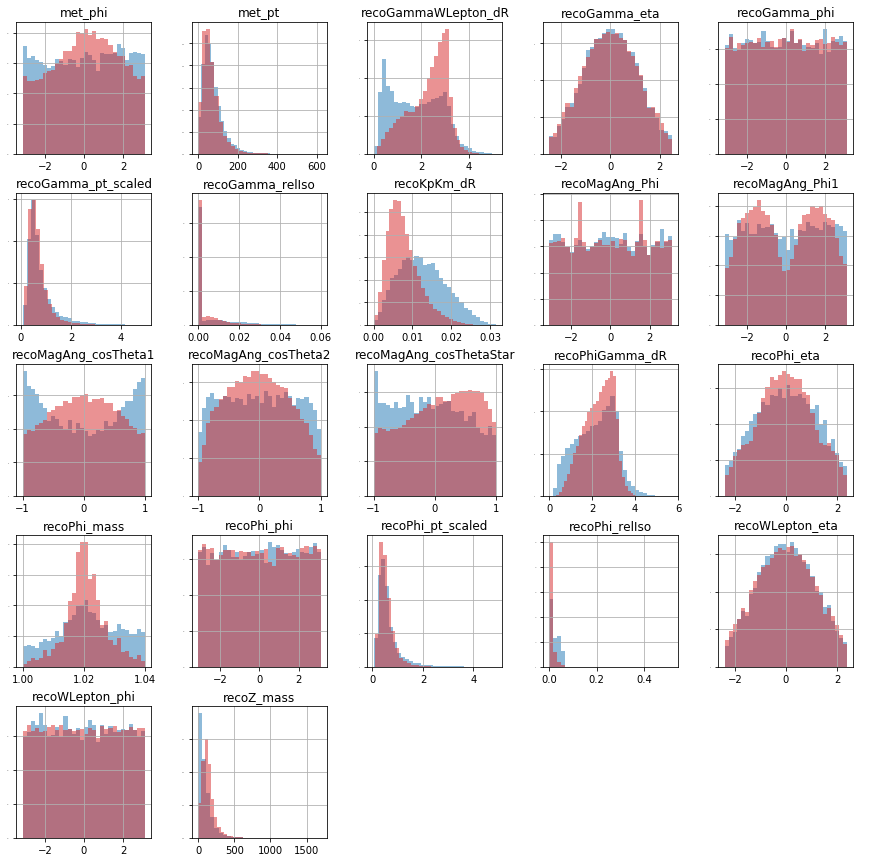
\includegraphics[width=.7\linewidth]{Dissertation/fig/bdt-training.png}
\end{center}
\caption{Preliminary histograms for every feature used to train the BDT. These were drawn before any weights are applied. ($H\rightarrow\phi\gamma$ analysis.)}
\label{fig:bdt-training}
\end{figure}

\begin{figure}[htb]
\begin{center}
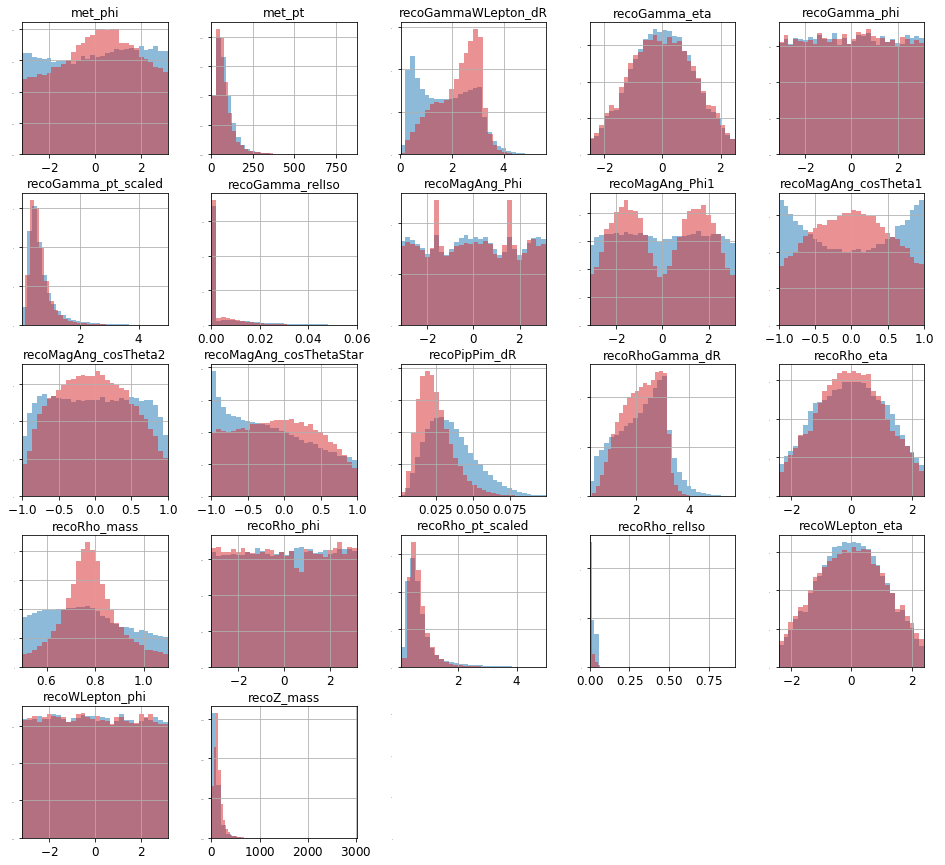
\includegraphics[width=.7\linewidth]{Dissertation/fig/bdt-training_rho.png}
\end{center}
\caption{Preliminary histograms for every feature used to train the BDT. These were drawn before any weights are applied. ($H\rightarrow\rho\gamma$ analysis.)}
\label{fig:bdt-training_rho}
\end{figure}

\begin{figure}[htb]
\begin{center}
\subfloat      {
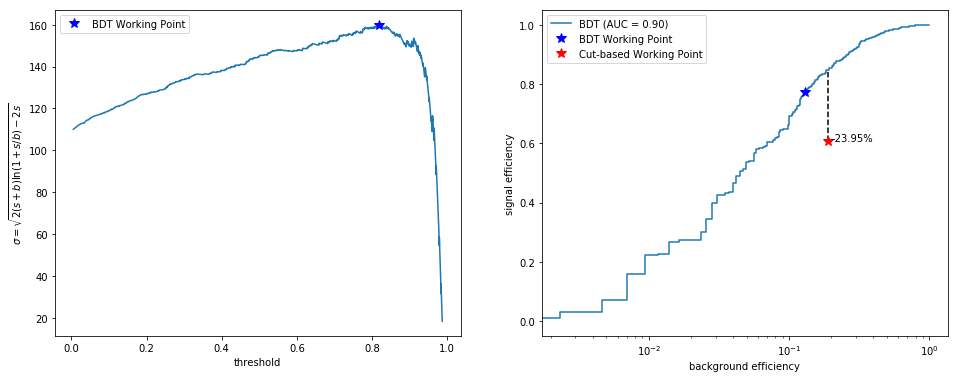
\includegraphics[width=.95\linewidth]{Dissertation/fig/bdt-vs-cuts.png}
}\\
\subfloat      {
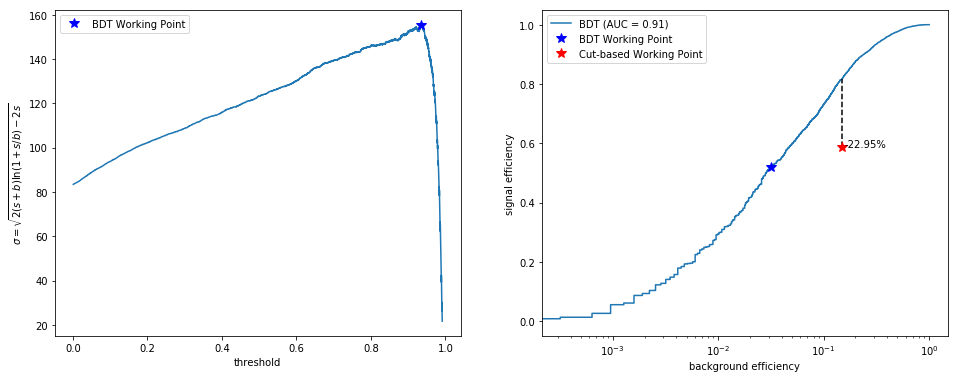
\includegraphics[width=.95\linewidth]{Dissertation/fig/bdt-vs-cuts_rho.png}
}
\end{center}
\caption{(Left) Expected significance ($\sigma$) versus BDT threshold value. (Right) Comparison between an optimal BDT working point and cut-based method plotted on top of the BDT's ROC curve. (Top) $H\rightarrow\phi\gamma$. (Bottom) $H\rightarrow\rho\gamma$.}
\label{fig:bdt-vs-cuts}
\end{figure}

\begin{figure}[htb]
\begin{center}
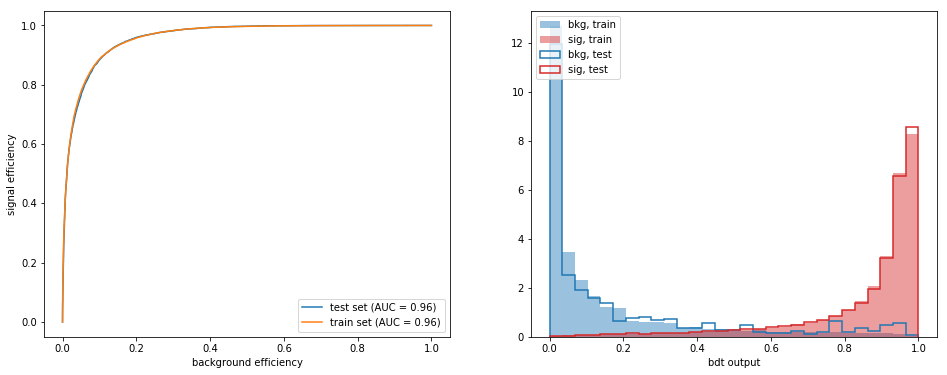
\includegraphics[width=.95\linewidth]{Dissertation/fig/bdt-performance_rho.png}
\end{center}
\caption{Left: ROC curve showing BDT testing (blue) and training (orange) performance. Right: Background (blue) and signal (red) distributions versus BDT score for testing (outline) and training (filled). ($H\rightarrow\rho\gamma$ analysis.)}
\label{fig:bdt-performance_rho}
\end{figure}

\begin{figure}[htb]
\begin{center}
\subfloat      {
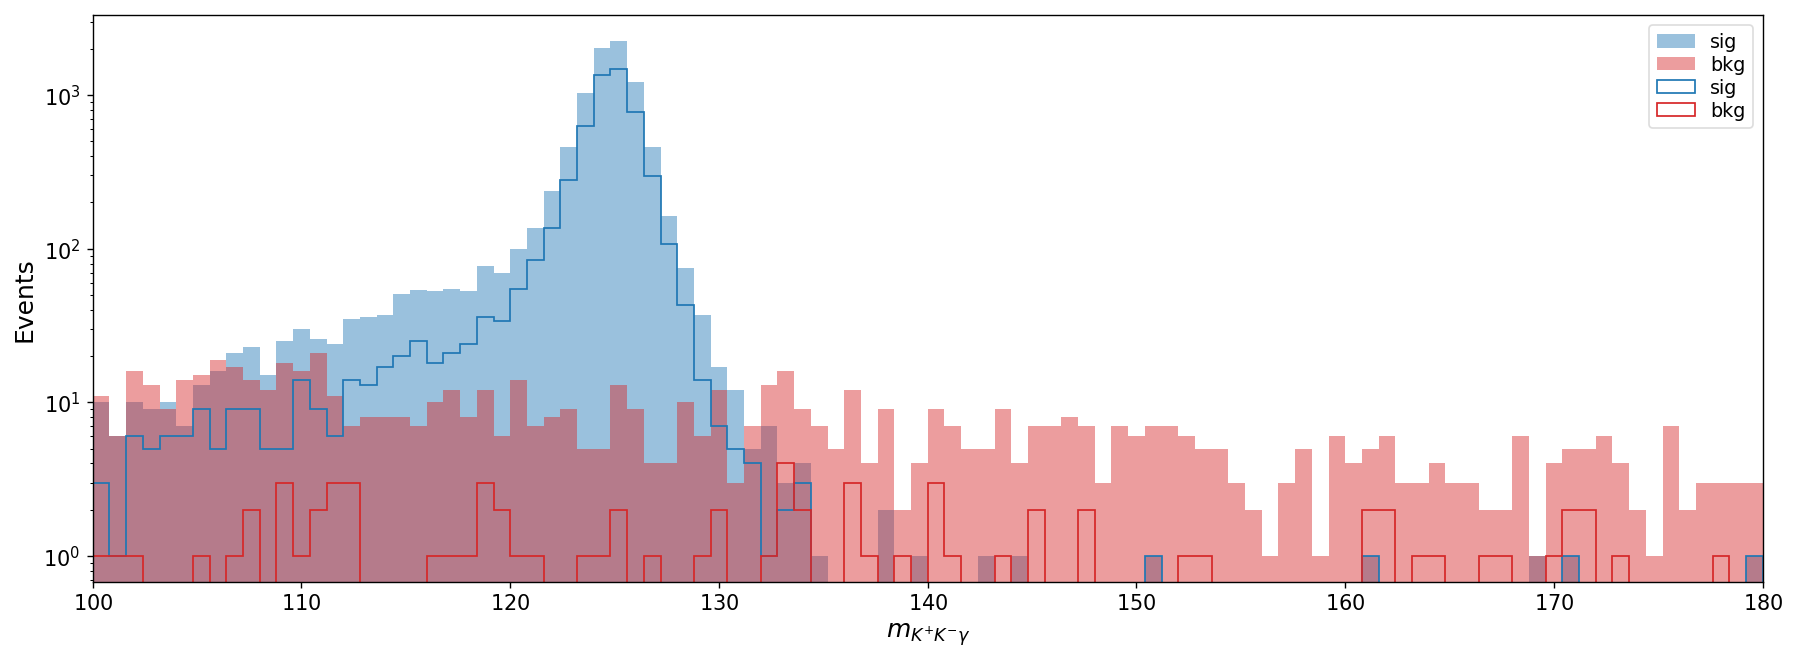
\includegraphics[width=.95\linewidth]{Dissertation/fig/bdt-bkgsculpt2.png}
}\\
\subfloat      {
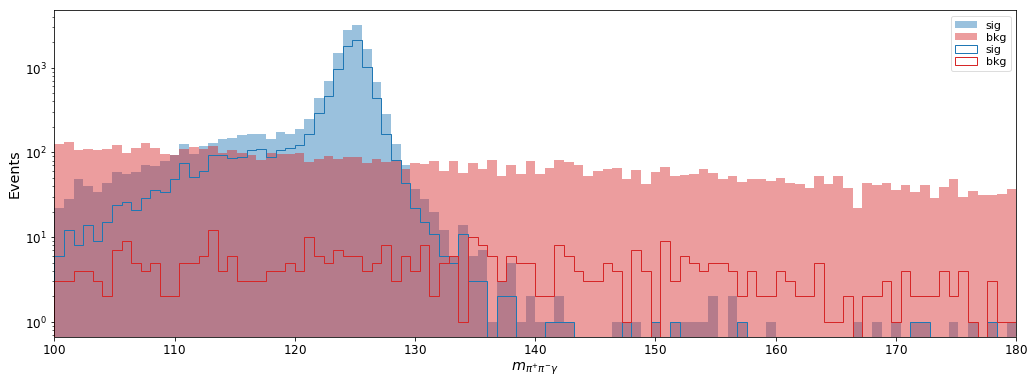
\includegraphics[width=.95\linewidth]{Dissertation/fig/bdt-bkgsculpt2_rho.png}
}
\end{center}
\caption{Reconstructed Higgs mass distribution for signal (blue) and background (red) before (filled) and after (outline) requiring $D > 0.9$. (Top) $H\rightarrow\phi\gamma$. (Bottom) $H\rightarrow\rho\gamma$.}
\label{fig:bdt-bkgsculpt2}
\end{figure}

\begin{figure}[htb]
\begin{center}
\subfloat      {
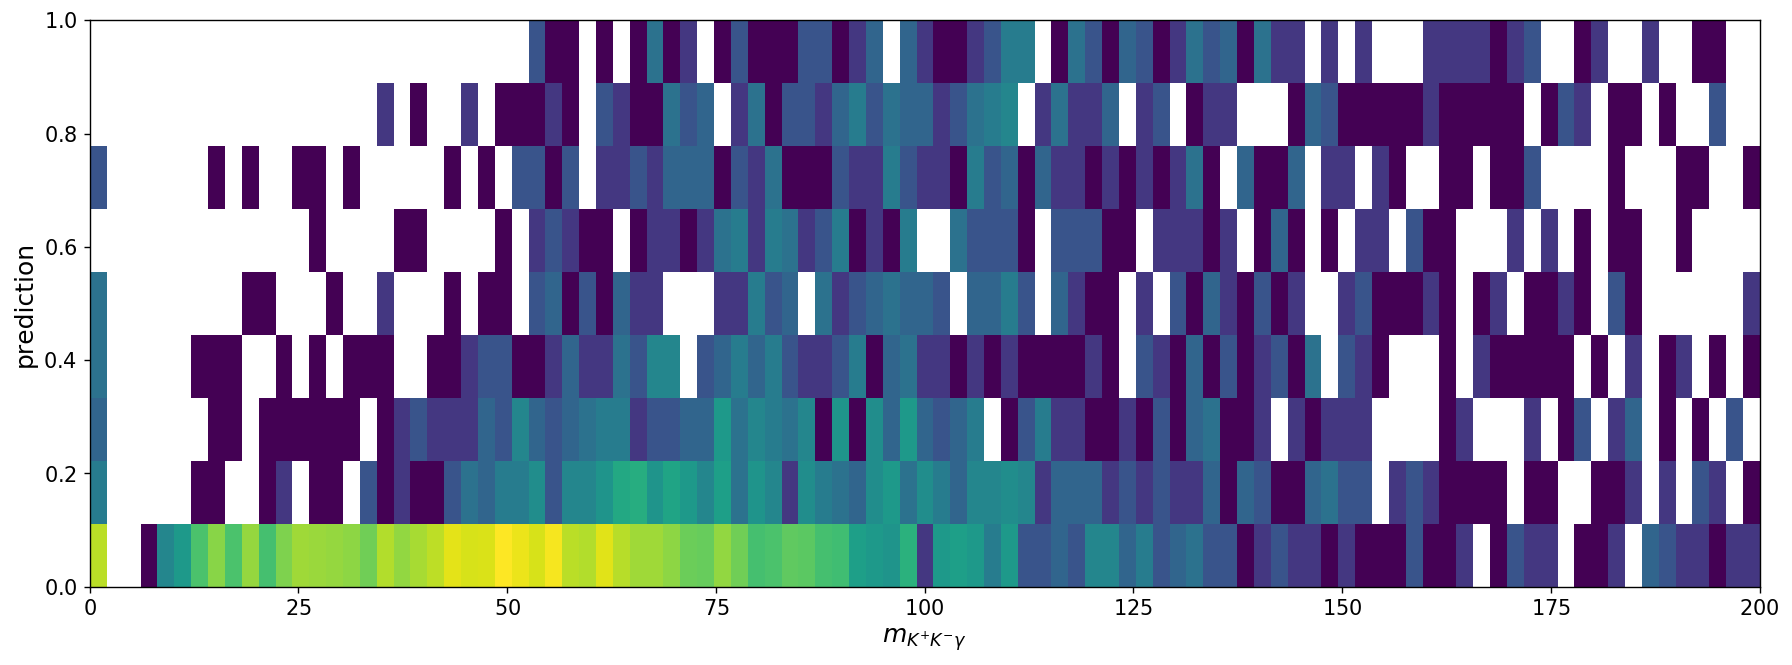
\includegraphics[width=.95\linewidth]{Dissertation/fig/bdt-bkgsculpt1.png}
}\\
\subfloat      {
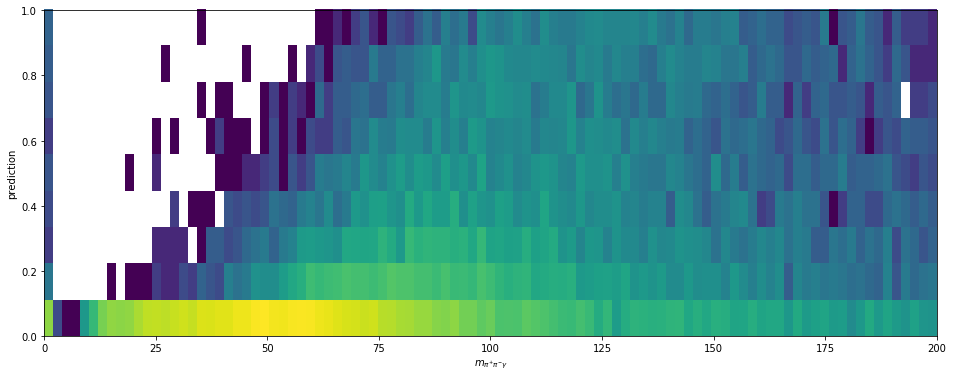
\includegraphics[width=.95\linewidth]{Dissertation/fig/bdt-bkgsculpt1_rho.png}
}
\end{center}
\caption{Plot of the BDT score versus the reconstructed Higgs mass. A heavy correlation between high score and the true Higgs mass would suggest background is being sculpted. (Top) $H\rightarrow\phi\gamma$. (Bottom) $H\rightarrow\rho\gamma$.}
\label{fig:bdt-bkgsculpt1}
\end{figure}

\begin{figure}[htb]
\begin{center}
\subfloat      {
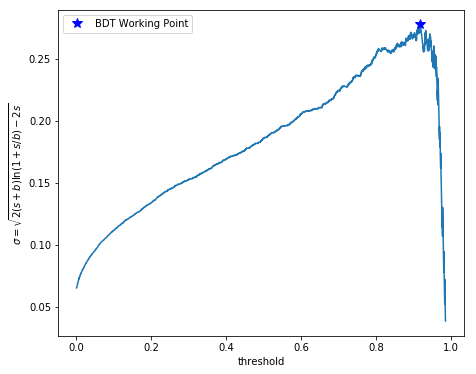
\includegraphics[width=.45\linewidth]{Dissertation/fig/data-expsig.png}
}\quad
\subfloat      {
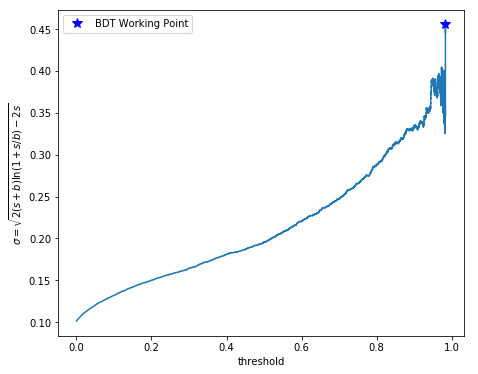
\includegraphics[width=.45\linewidth]{Dissertation/fig/data-expsig_rho.png}
}
\end{center}
\caption{Expected significance ($\sigma$) versus BDT threshold. (Left) $H\rightarrow\phi+\gamma$ analysis. (Right) $H\rightarrow\rho+\gamma$ analysis.}
\label{fig:bdt-data-expsig}
\end{figure}

\chapter{Technical Details}
\begin{section}{CMS Coordinate System}\label{appendix:cms-coords}

In the CMS Coordinate system, the $z$-axis is aligned along the beampipe, therefore running parallel to the barrel and perpendicular to the endcap of the detector. The $x$-axis points radially towards the center of the LHC, and the y-axis points orthogonal to $x$ and $z$. The azimuthal angle $\varphi$ is defined about the $z$-axis, as in cylindrical coordinates, and the pseudo-rapidity $\eta$ is defined as

\begin{equation}
    \eta \equiv -\ln{\bigg[ \tan{\bigg( \frac{\theta}{2} \bigg)} \bigg]}
\end{equation}

\noindent where $\theta$ is the angle between the particle three-momentum and positive $z$-axis. See Figure \ref{fig:cms-coords} for a visualization of this coordinate system.

\begin{figure}[htb]
\begin{center}
\tdplotsetmaincoords{75}{50} % to reset previous setting
\begin{tikzpicture}[scale=2.7,tdplot_main_coords,rotate around x=90]
 
  % variables
  \def\rvec{1.2}
  \def\thetavec{40}
  \def\phivec{70}
  \def\R{1.1}
  \def\w{0.3}
 
  % axes
  \coordinate (O) at (0,0,0);
  \draw[thick,->] (0,0,0) -- (1,0,0) node[below left]{$x$};
  \draw[thick,->] (0,0,0) -- (0,1,0) node[below right]{$y$};
  \draw[thick,->] (0,0,0) -- (0,0,1) node[below right]{$z$};
  \tdplotsetcoord{P}{\rvec}{\thetavec}{\phivec}
 
  % vectors
  \draw[->,red] (O) -- (P) node[above left] {$P$};
  \draw[dashed,red] (O)  -- (Pxy);
  \draw[dashed,red] (P)  -- (Pxy);
  \draw[dashed,red] (Py) -- (Pxy);
 
  % circle - LHC
  \tdplotdrawarc[thick,rotate around x=90,black!70!blue]{(\R,0,0)}{\R}{0}{360}{}{}
 
  % compass - the line between CMS and ATLAS has a ~12° declination (http://googlecompass.com)
  \begin{scope}[shift={(1.1*\R,0,1.65*\R)},rotate around y=12]
    \draw[<->,black!50] (-\w,0,0) -- (\w,0,0);
    \draw[<->,black!50] (0,0,-\w) -- (0,0,\w);
    \node[above left,black!50,scale=0.6] at (-\w,0,0) {N};
  \end{scope}
 
  % nodes
  \node[left,align=center] at (0,0,1.1) {Jura};
  \node[right] at (\R,0,0) {LHC};
  \fill[radius=0.8pt,black!20!red]
    (O) circle node[left=4pt,below=2pt] {CMS};
  \draw[thick] (0.02,0,0) -- (0.5,0,0); % partially overdraw x-axis and CMS point
  \fill[radius=0.8pt,black!20!blue]
    (2*\R,0,0) circle
    node[right=4pt,below=2pt,scale=0.9] {ATLAS};
  \fill[radius=0.8pt,black!10!orange]
    ({\R*sqrt(2)/2+\R},0,{ \R*sqrt(2)/2}) circle % 45 degrees from ATLAS
    node[left=2pt,below=2pt,scale=0.8] {ALICE};
  \fill[radius=0.8pt,black!60!green]
    ({\R*sqrt(2)/2+\R},0,{-\R*sqrt(2)/2}) circle % 45 degrees from ATLAS
    node[below=2pt,right=2pt,scale=0.8] {LHCb};
 
  % arcs
  \tdplotdrawarc[->]{(O)}{0.2}{0}{\phivec}
    {above=2pt,right=-1pt,anchor=mid west}{$\varphi$}
  \tdplotdrawarc[->,rotate around z=\phivec-90,rotate around y=-90]{(0,0,0)}{0.5}{0}{\thetavec}
    {anchor=mid east}{$\eta$}
 
\end{tikzpicture}
\end{center}
\caption{Diagram of CMS coordinate system.}
\label{fig:cms-coords}
\end{figure}

\end{section}

\begin{section}{Kinematic Variable Definitions}
The following quantities are defined using the CMS Coordinate System defined in Appendix A.1. First, it is useful to define ``transverse" components (denoted as $A_{T}$ for a three or four-vector quantity A) to be the spatial $x$ and $y$-components of a given variable. Additionally, $\Delta R$ between two particles $x_1, x_2$ is defined as
\begin{equation}
    \Delta R(x_1, x_2) = \sqrt{\Delta\varphi(x_1, x_2)^{2}+\Delta\eta(x_1, x_2)^{2}}
\end{equation}
\noindent where $\Delta\eta(x_1, x_2) = \eta(x_2)-\eta(x_1)$, and $\Delta\varphi(x_1, x_2) = |\varphi(x_2) - \varphi(x_1)|$ is the \textit{inner} angle between the $x_1$ and $x_2$ three-momenta), such that $\Delta\varphi \in [0, 2\pi]$. Then, the isolation $I$ of a particle $x$ is defined as the sum of transverse momentum $p_{T}$ in a cone of $\Delta R < 0.4$\cite{cite-iso-dR} around that particle. Finally, the ``relative" isolation $I_{rel}$ of a particle $x$ is defined as:
\begin{equation}
    I_{rel}(x) = \frac{I(x)}{p_{T}(x)}
\end{equation}
\end{section}

\begin{section}{Boosted Decision Trees}
A Boosted Decision Tree (BDT) is simply an extension of a decision tree, which is can be visualized as follows: starting from a single ``node," two ``branches" emerge; at the end of each branch, there is another node that also joins two branches, and so on. In this picture, each node is a binary decision (i.e. $A > B$, $C == D$, etc.) and the two branches joined by each node represent the path ``traveled" by data should it pass or fail -- hence \textit{two} branches -- the condition. The tree may be optimized by recursively adding nodes and adjusting the ``splits" (the exact value over which the input is split) at each node until some given condition is met such that an optimal configuration is reached. This is essentially an accurate representation of the classical, ``cut-based" analysis that has been performed in High Energy for decades, where physicists filter out everything they are not looking for (background) with the hope that what they are looking for (signal) remains after the surrounding noise is cleared. A similar (both in practice and results) optimization of this technique is achieved by a combination of educated insight and trail and error. Thus, the computational method of the decision tree fits into the workflow of a High Energy physics analysis, but a decision tree is not an exceptionally powerful classifier on its own. However, they can be ``boosted" by creating several decision trees, collecting their output, and calculating a value called a ``determinant" (henceforth referred to as $D$), forming a stronger classifier from the collection of weak ones. The exact process of constructing and optimizing a BDT is dependent on the particular algorithm used and is beyond the scope of this paper.

\begin{figure}[htb]
\begin{center}
\begin{tabular}{p{.25\linewidth} p{.75\linewidth}}
\toprule
Variable & Definition \\
\midrule
\verb|objective| & Learning objective. (`binary:logistic': logistic regression for binary classification, output probability) \\
\verb|eta| & Step size shrinkage used in update to prevents overfitting. (range: $[0,1]$) \\
\verb|max_depth| & Maximum depth of a tree. Increasing this value will make the model more complex and more likely to overfit. (range: $[0,\infty]$) \\
\verb|verbosity| & Verbosity of printing messages. Valid values are 0 (silent), 1 (warning), 2 (info), 3 (debug). \\
\verb|nthread| & Number of parallel threads used to run XGBoost. \\
\verb|eval_metric| & Evaluation metrics for validation data. (`auc': Area under the curve) \\
\verb|subsample| & Subsample ratio of the training instances. (range: $(0,1]$) \\
\verb|alpha| & L1 regularization term on weights. Increasing this value will make model more conservative. \\
\verb|gamma| & Minimum loss reduction required to make a further partition on a leaf node of the tree. The larger \verb|gamma| is, the more conservative the algorithm will be. (range: $[0,\infty]$) \\
\verb|lambda| & L2 regularization term on weights. Increasing this value will make model more conservative. Normalized to number of training examples. \\
\verb|min_child_weight| & Minimum sum of instance weight (hessian) needed in a child. The larger \verb|min_child_weight| is, the more conservative the algorithm will be. \\
\verb|colsample_bytree| & Subsample ratio of columns when constructing each tree. Subsampling occurs once for every tree constructed. \\
\bottomrule
\end{tabular}
\end{center}
\caption{XGBoost BDT hyperparameters\cite{cite-xgboost-params}.}
\label{fig:bdt-knobs}
\end{figure}
\end{section}